\documentclass[tikz,border=3.14mm]{standalone}
\usetikzlibrary{positioning,calc,shapes.geometric}
\begin{document}
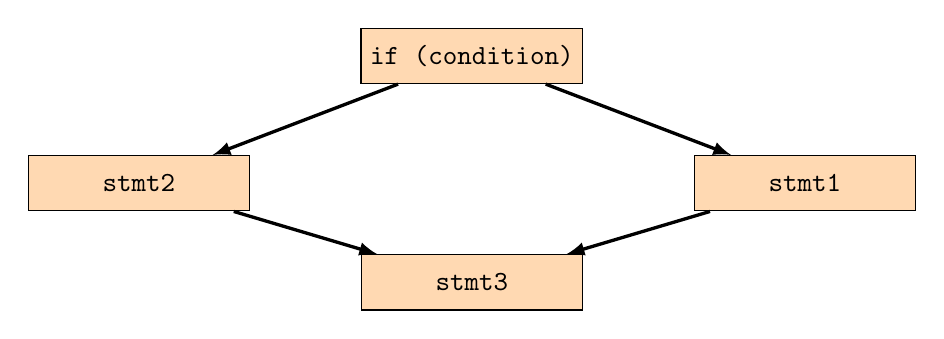
\begin{tikzpicture}[node distance = 9mm and 14mm,
  nodes= {draw, minimum width=8em, minimum height=2em,
    font=\ttfamily},
  startstop/.style = {fill=red!30, rounded corners},
  process/.style = {fill=orange!30},
  io/.style = {fill=blue!30,
    trapezium, trapezium stretches body,
    trapezium left angle=70, trapezium right angle=110},
  decision/.style = {fill=green!30, diamond, aspect=1.5},
  exp/.style={draw=none,font=\sffamily,minimum width=1em},
  arr/.style = {very thick,-latex}
  ]
  \node (if) [process] {if (condition)};
  \node (true-bb)  [process, below right=of if] {stmt1};
  \node (false-bb) [process, below left=of if]  {stmt2};
  \node (end) [process, below=of $(true-bb)!0.5!(false-bb)$] {stmt3};

  \draw[arr] (if) -- (true-bb);
  \draw[arr] (if) -- (false-bb);
  \draw[arr] (true-bb) -- (end);
  \draw[arr] (false-bb) -- (end);
\end{tikzpicture}
\end{document}
